\documentclass[11pt,a4paper]{article}
\usepackage[margin=2cm]{geometry}
\usepackage{lmodern}
\usepackage[T1]{fontenc}
\usepackage{amsmath,amssymb}
\usepackage{booktabs,array,tabularx,xltabular}
\usepackage{enumitem}
\usepackage{xcolor}
\usepackage[most]{tcolorbox}
\usepackage{titlesec}
\usepackage{graphicx}
\usepackage{float}
\usepackage{needspace}
\usepackage[font=small,labelfont={bf,color=headblue},skip=4pt]{caption}
\usepackage[colorlinks=true,linkcolor=black,urlcolor=blue!50!black]{hyperref}

% ---- one look for the whole report -------------------------------------------
\definecolor{headblue}{RGB}{38,70,120}
\titleformat{\section}{\Large\bfseries\color{headblue}}{\thesection}{0.8em}{}[{\color{black}\titlerule}]
\titleformat{\subsection}{\large\bfseries\color{headblue}}{\thesubsection}{0.8em}{}
\titlespacing*{\section}{0pt}{12pt}{6pt}
\titlespacing*{\subsection}{0pt}{8pt}{3pt}
\setlength{\parindent}{0pt}
\setlength{\parskip}{4pt}
\AtBeginDocument{\setlength{\abovedisplayskip}{4pt}\setlength{\belowdisplayskip}{4pt}}
\setlist{itemsep=1pt,topsep=2pt}
\setlength{\emergencystretch}{3em}
\setlength{\LTpre}{2pt}\setlength{\LTpost}{2pt}
\setlength{\textfloatsep}{10pt}
\renewcommand{\arraystretch}{1.1}
\allowdisplaybreaks

\newcommand{\mdesc}[1]{\par{\textit{Meaning:} #1}\par}
\newtcolorbox{objbox}{colback=blue!3,colframe=headblue!60,boxrule=0.5pt,arc=2mm,left=2mm,right=2mm,top=1mm,bottom=1mm}

\begin{document}

\begin{center}
{\LARGE\bfseries\color{headblue} EV Charging Network Optimisation}\\[6pt]
{\normalsize CP 320 Operations Research for Mobility, course project report}\\[2pt]
{\normalsize Yakshith Maddineni (SR 26080) \quad\textperiodcentered\quad Kartikeya Gaur (SR 26371)}\\[2pt]
{\normalsize 23 October 2026}
\end{center}

% Sections 1-5: the main formulation, exactly as in ../main_formulation.tex.
% formulation_body.tex is generated by prepare_report.py; edit main_formulation.tex, then re-run it.
% Generated by prepare_report.py from ../main_formulation.tex - do not edit here.
%=====================================================================
\section{Problem Statement}

Given a small road network, the network operator wants to assign each EV with its respective demand either to a fixed charging station or a mobile charging station.

\hspace{1.5em}During the time interval $[0,T]$ a set of parked EVs raise charging requests. Each request must be served by exactly one resource: either the EV drives itself to a fixed charging station (FCS, 2 guns of 22\,kW each), or a mobile charging van (MCS) leaves the depot, drives to the EV, charges it (one EV at a time) and moves on, returning to the depot by $T$.

We decide -
\begin{enumerate}[itemsep=2pt]
  \item Who serves each EV.
  \item The order in which each van visits its EVs.
  \item The time every charging session starts.
\end{enumerate}

\begin{objbox}
{\color{headblue}\textbf{Our Objective}}\\
Minimize the total operating cost and penalty for customer inconvenience.
\end{objbox}

%=====================================================================
\section{Assumptions}
\begin{enumerate}[itemsep=2pt]
  \item All requests of the planning period are known at time 0; request $i$ becomes active at $r_i$ (request release time). All times are non-negative real numbers, measured in minutes, in $[0,T]$.
  \item An EV served by an FCS drives there itself (one way) on its own battery, waits for a free gun, and stays until charged. An EV can only use an FCS within its remaining range.
  \item An EV served by an MCS stays parked at its location; the van comes to it.
  \item Each FCS gun and each MCS charges one EV at a time, with no pre-emption.
  \item A van's driving energy and delivered energy come from the same battery; there is no recharging of the van during the peak.
  \item Every request must be fully charged by $T$ (hard).
  \item Charging power is constant.
\end{enumerate}

%=====================================================================
\section{Sets, parameters and decision variables}

\subsection*{Sets}
\begin{xltabular}{\textwidth}{@{}>{\raggedright\arraybackslash}p{4.6cm}X@{}}
\toprule
\textbf{Notation} & \textbf{Description} \\
\midrule
$I=\{1,\dots,n\}$ & Set of EV charging requests. \\[2pt]
$F$,\ \ $|F|=12$ (or $24$) & Set of fixed charging stations (FCS). Dataset: 12 stations in the 100-EV files, 24 in the 200-EV files. \\[2pt]
$G_f$,\ \ $|G_f|=2$ & Set of guns (charging points) at FCS $f$, with $|G_f|=2$. Define $G=\bigcup_{f\in F}G_f$, and let $f(g)$ denote the station associated with gun $g$. Dataset: $|G|=24$ (or $48$). \\[2pt]
$F_i=\{f\in F: d_{if}\le R_i\}$ & Set of FCS that EV $i$ can reach given its remaining range. \\[2pt]
$G_i=\bigcup_{f\in F_i}G_f$ & Set of guns that EV $i$ can use. \\[2pt]
$M$,\ \ $|M|=5$ (or $12$) & Set of mobile charging vans. Dataset: 5 vans in the 100-EV files, 12 in the 200-EV files, for every instance size $n$. \\[2pt]
$0,\ n+1$ & Start and end depot nodes, respectively, representing the same physical location. (assumed single depot) \\[2pt]
$N=\{0\}\cup I\cup\{n+1\}$ & Set of routing nodes. \\[2pt]
$A$ & Set of allowed van-routing arcs, defined as \newline
$A=\{(i,j): i\in\{0\}\cup I,$\newline
\hspace*{3.2em}$j\in I\cup\{n+1\},$\newline
\hspace*{3.2em}$i\ne j,\ (i,j)\ne(0,n+1)\}$. \\[2pt]
$P_g=\{(i,j)\in I^2: i<j,\ g\in G_i\cap G_j\}$ & Set of EV pairs that could be assigned to the same gun $g$ (and must then be sequenced). \\[2pt]
$G^{+}=\{g\in G: g\in G_i \text{ for some } i\in I\}$ & Set of guns that at least one EV can reach. \\
\bottomrule
\end{xltabular}\addtocounter{table}{-1}

\subsection*{Parameters}
{\small
\begin{xltabular}{\textwidth}{@{}>{\raggedright\arraybackslash}p{4.6cm}X@{}}
\toprule
\textbf{Notation} & \textbf{Description} \\
\midrule
$E_i\in[10,40]$ & Energy demand of EV $i$ (kWh). Dataset: Solomon DEMAND (1--50) mapped linearly, $E_i=10+30\,(\text{DEMAND}_i-1)/49$. \\[2pt]
$r_i$ & Request (release) time (minutes). [$r_i=0$ for static demand] Dataset: Solomon READY TIME, unchanged. \\[2pt]
$R_i$ & Remaining driving range of EV $i$ (km). Dataset: uniform on $[5,40]$; for 15\,\% of the EVs (``stranded'') $R_i$ is 20--80\,\% of the distance to their nearest FCS, so $F_i=\emptyset$ and only a van can serve them. \\[2pt]
$w_i=1+\kappa\Big(1-\dfrac{R_i}{R_{\max}}\Big)$,\newline $\kappa=2$ & Priority weight of EV $i$ ($w_i\ge1$): EVs with less remaining range are more urgent and weigh more. $R_{\max}=\max_{i\in I}R_i$; $\kappa\ge0$ sets how strongly urgency counts ($\kappa=0$: all EVs weigh 1; $\kappa=2$: an EV with almost no range weighs about 3). Dataset: $\kappa=2$, so $w_i\in[1,3]$. \\[2pt]
$P^{\mathrm F}=22,\ P^{\mathrm M}=30$ & Charging power of an FCS gun and an MCS (kW). \\[2pt]
$\tau^{\mathrm F}_i=\dfrac{60\,E_i}{P^{\mathrm F}},\ \tau^{\mathrm M}_i=\dfrac{60\,E_i}{P^{\mathrm M}}$ & Charging duration of EV $i$ at an FCS and by an MCS, respectively (minutes). Dataset: $\tau^{\mathrm F}_i=60E_i/22\in[27,109]$, $\tau^{\mathrm M}_i=60E_i/30\in[20,80]$. \\[2pt]
$d_{if},\ t_{if}=\dfrac{60\,d_{if}}{v}$ & Shortest-path distance (km) and travel time (minutes) from EV $i$ to FCS $f$. \\[2pt]
$d_{ij},\ t_{ij}=\dfrac{60\,d_{ij}}{v}$ & Shortest-path distance (km) and travel time (minutes) between routing nodes. Dataset: $d=1.3\times0.2\times$ (straight-line distance in Solomon grid units), i.e.\ 1 grid unit $=0.2$\,km and a road detour factor of 1.3. \\[2pt]
$v=15.6$ & Travel speed (km/h), assumed identical for all vehicles. Dataset: $v=60\times0.2\times1.3=15.6$\,km/h, so that $t$ in minutes equals the straight-line grid distance (Solomon's rule). \\[2pt]
$B_m=150$ & Usable battery capacity of MCS $m$ (kWh). \\[2pt]
$Q_m=6$ & Maximum number of EVs MCS $m$ may serve during the planning period. \\[2pt]
$\beta=0.25$ & Van driving energy consumption (kWh/km). \\[2pt]
$\eta=0.9$ & MCS charging efficiency (battery to EV), $\eta\in(0,1]$. \\[2pt]
$T$ & Length of the planning period (minutes). Dataset: Solomon's depot due date, unchanged. 100-EV files: C1 1236, C2 3390, R1 230, R2 1000, RC1 240, RC2 960. 200-EV files: C1 1351, C2 3598, R1 634, R2 2535, RC1 634, RC2 2535. \\[2pt]
$c^{\mathrm{EV}}=4,\ c^{\mathrm M}=15$ & Cost per kilometre of EV driving and van driving, respectively (Rs/km). \\[2pt]
$c^{\mathrm F}_m=1500$ & Fixed dispatch cost of van $m$ (driver, depreciation) (Rs). \\[2pt]
$\pi^{\mathrm F}=8.7,\ \pi^{\mathrm M}=10.7$ & Cost per kWh of grid energy at an FCS and energy stored in a van battery, respectively (Rs/kWh). \\[2pt]
$c^{\mathrm W}=200/60\approx3.33$ & Inconvenience cost per minute of time lost by the driver (Rs/minute; an hourly value of time of Rs\,200 divided by 60). \\[2pt]
$M^{\mathrm M}_{ij}=T+\tau^{\mathrm M}_i+t_{ij}$ & Big-$M$ constant for van sequencing constraints (minutes). \\[2pt]
$M^{\mathrm F}_i=T+\tau^{\mathrm F}_i$ & Big-$M$ constant for gun sequencing constraints (minutes). \\
\bottomrule
\end{xltabular}\addtocounter{table}{-1}}

\textbf{Units.} Energy is in kWh, power in kW, distance in km and speed in km/h; every time quantity ($r_i$, $T$, $S_i$, $C_i$, $\tau$, $t$, big-$M$) is in minutes. Since kWh/kW and km/(km/h) give hours, charging and travel times are multiplied by 60. With $c^{\mathrm W}$ per minute, the term $c^{\mathrm W}w_i(C_i-r_i)$ is in currency units, like all other terms of $Z$. In the dataset the currency is Indian rupees (Rs).

\textbf{Values.} An ``$=$'' in the tables gives the value used in every file of the EV-Solomon dataset (\texttt{dataset\_ev\_solomon}); a value in parentheses after ``or'' applies to the 200-EV (Gehring--Homberger) files. $T$, $r_i$, $E_i$ and the locations come from the Solomon / Gehring--Homberger source files; all other values are our assumptions.

\subsection*{Decision Variables}
\begin{xltabular}{\textwidth}{@{}>{\raggedright\arraybackslash}p{4.6cm}X@{}}
\toprule
\textbf{Notation} & \textbf{Description} \\
\midrule
$y_{ig}\in\{0,1\}$ & 1 if EV $i$ is charged at gun $g\in G_i$; 0 otherwise. \\[2pt]
$z_{im}\in\{0,1\}$ & 1 if EV $i$ is served by van $m$; 0 otherwise. \\[2pt]
$x_{ijm}\in\{0,1\}$ & 1 if van $m$ traverses arc $(i,j)\in A$; 0 otherwise. \\[2pt]
$u_m\in\{0,1\}$ & 1 if van $m$ is dispatched; 0 otherwise. \\[2pt]
$o_{ij}\in\{0,1\}$ & For EV pairs $i<j$ sharing a gun, 1 if EV $i$ is charged before EV $j$; 0 otherwise. \\[2pt]
$S_i\ge0$ & Start time of EV $i$'s charging session, irrespective of the resource used (minute). \\
\bottomrule
\end{xltabular}\addtocounter{table}{-1}

Short-hands:
\begin{gather*}
Y_{if}=\sum_{g\in G_f}y_{ig}\quad\text{(EV $i$ goes to FCS $f$)},\\
C_i=S_i+\tau^{\mathrm F}_i\sum_{g\in G_i}y_{ig}+\tau^{\mathrm M}_i\sum_{m\in M}z_{im}\quad\text{(completion time)}.
\end{gather*}
Because exactly one of the $y/z$ terms equals 1, $C_i$ is the start time plus the duration on the chosen resource.

%=====================================================================
\section{Objective}

\begin{equation}
\begin{aligned}
\min\ Z \;=\;& \underbrace{c^{\mathrm{EV}}\sum_{i\in I}\sum_{f\in F_i}d_{if}Y_{if}}_{Z_1:\ \text{EV driving}}
+\underbrace{c^{\mathrm M}\sum_{m\in M}\sum_{(i,j)\in A}d_{ij}x_{ijm}}_{Z_2:\ \text{van driving}}
+\underbrace{\sum_{m\in M}c^{\mathrm F}_mu_m}_{Z_3:\ \text{van dispatch}}\\
&+\underbrace{\pi^{\mathrm F}\sum_{i\in I}\sum_{g\in G_i}E_iy_{ig}+\pi^{\mathrm M}\sum_{i\in I}\sum_{m\in M}\frac{E_i}{\eta}z_{im}}_{Z_4:\ \text{energy}}\\
&+\underbrace{c^{\mathrm W}\sum_{i\in I}w_i(C_i-r_i)}_{Z_5:\ \text{inconvenience}}\,.
\end{aligned}\label{eq:obj}
\end{equation}

$Z_1$ \textbf{EV driving.} Distance each FCS user drives to its station. It pushes EVs towards the nearest FCS with a free gun: a closer station is cheaper, and a closer station also starts charging earlier, which lowers $Z_5$.

$Z_2$ \textbf{van driving.} Total km of all van routes (fuel/wear/driver time per km).

$Z_3$ \textbf{dispatch.} Fixed cost of every van that leaves the depot; with $Z_2$ this is the ``operating cost of MCS'' in the problem statement.

$Z_4$ \textbf{energy.} The same kWh cost different amounts by resource: grid price at an FCS, versus van energy which is dearer per kWh and loses $1-\eta$ in transfer. This is the main reason an MCS is not used for everyone. Energy is included because it is a real operating cost of the operator (the problem statement's list of cost terms says the cost ``may include'' them, so the list is not exhaustive) and because it is the main per-EV cost difference between the two resources: a van must draw $E_i/\eta$ to deliver $E_i$, at a higher price per kWh. Without $Z_4$ the model would see van energy as free and overuse vans whenever they reduce waiting. (If drivers pay for FCS energy themselves, only the van term is an operator cost.)

$Z_5$ \textbf{inconvenience.} $C_i-r_i$ is the time (in minutes) from request until the car is fully charged: for an FCS user it is driving + queueing at the gun + charging; for an MCS user it is waiting for the van + charging. Multiplying by $w_i$ gives priority: low-range (urgent) EVs cost more per minute of delay, so the model serves them first. With $w_i=1+\kappa(1-R_i/R_{\max})$, a minute of waiting for an EV with almost no range left costs up to $1+\kappa$ times as much as for the EV with the most range; this is the only place $w_i$ enters the model. ($\sum_i w_ir_i$ is a constant and can be dropped when solving.)

All terms are in currency units; the weight $c^{\mathrm W}$ converts time into money and can be varied to trade cost against service.

%=====================================================================
\section{Constraints}

\subsection{Assignment}
\begin{equation}
\sum_{g\in G_i}y_{ig}+\sum_{m\in M}z_{im}=1\qquad\forall i\in I \label{eq:assign}
\end{equation}
\mdesc{Every request is served by exactly one resource: one gun of one reachable FCS, or one van. If EV $i$ reaches no FCS ($G_i=\emptyset$) it is forced onto a van, which is how range-critical EVs are protected.}

\subsection{Fixed charging stations (continuous time)}
\begin{equation}
S_i\ \ge\ r_i+\sum_{f\in F_i}t_{if}\,Y_{if}\qquad\forall i\in I \label{eq:fcsarr}
\end{equation}
\mdesc{An FCS user cannot start before it has been requested and has driven to its station. For an MCS user the sum is zero and this becomes $S_i\ge r_i$.}

\begin{align}
S_j &\ge S_i+\tau^{\mathrm F}_i-M^{\mathrm F}_i\,(3-y_{ig}-y_{jg}-o_{ij}) && \forall g\in G,\ (i,j)\in P_g \label{eq:disj1}\\
S_i &\ge S_j+\tau^{\mathrm F}_j-M^{\mathrm F}_j\,(2-y_{ig}-y_{jg}+o_{ij}) && \forall g\in G,\ (i,j)\in P_g \label{eq:disj2}
\end{align}
\mdesc{No two EVs overlap on the same gun. If both $i$ and $j$ use gun $g$ ($y_{ig}=y_{jg}=1$), then either $o_{ij}=1$ and \eqref{eq:disj1} forces $j$ to start after $i$ has finished, or $o_{ij}=0$ and \eqref{eq:disj2} forces the reverse. If either is not on $g$ the big-$M$ switches both constraints off. With two guns per station this is exactly ``at most 2 EVs charging at an FCS at any moment'', without any time grid. $M^{\mathrm F}_i=T+\tau^{\mathrm F}_i$ is enough because $0\le S_i\le T$.}

\begin{equation}
\sum_{i\in I}\tau^{\mathrm F}_i\,y_{ig}\ \le\ T-\min_{i:\,g\in G_i}\Big(r_i+t_{if(g)}\Big)\qquad\forall g\in G^{+} \label{eq:gunload}
\end{equation}
\mdesc{Valid inequality (implied by the others, added to tighten the LP relaxation): the total charging time on one gun cannot exceed the time it is available. It also gives a cheap aggregate capacity model if the instance is too large for the sequencing constraints. It is written only for guns in $G^{+}$: if no EV can reach gun $g$, the set $\{i: g\in G_i\}$ is empty, its minimum is undefined, and the gun has no $y_{ig}$ variables anyway, so nothing is lost.}


\begin{equation}
\sum_{i\in I}y_{ig_1}\ \ge\ \sum_{i\in I}y_{ig_2}\qquad\forall f\in F,\ G_f=\{g_1,g_2\} \label{eq:gunsym}
\end{equation}
\mdesc{Symmetry breaking: the two guns of a station are identical, so let gun 1 carry at least as many EVs as gun 2. Optional; it removes mirror solutions and speeds up branch-and-bound.}

\subsection{MCS routing}
\begin{align}
\sum_{j:(0,j)\in A}x_{0jm} &= u_m && \forall m\in M \label{eq:out}\\
\sum_{i:(i,n+1)\in A}x_{i,n+1,m} &= u_m && \forall m\in M \label{eq:in}\\
\sum_{i:(i,j)\in A}x_{ijm} &= z_{jm} && \forall j\in I,\ m\in M \label{eq:flowin}\\
\sum_{k:(j,k)\in A}x_{jkm} &= z_{jm} && \forall j\in I,\ m\in M \label{eq:flowout}
\end{align}
\mdesc{\eqref{eq:out}--\eqref{eq:in}: a dispatched van leaves the depot once and returns once; an unused van does neither. \eqref{eq:flowin}--\eqref{eq:flowout}: every EV assigned to van $m$ is entered once and left once by that van, i.e.\ visited exactly once; EVs not on $m$ are not touched by it. Together they make each van's arcs one path $0\to\cdots\to n+1$ (plus possible cycles, removed by \eqref{eq:seq}).}

\subsection{MCS capacity and battery}
\begin{align}
\sum_{i\in I}z_{im} &\le Q_m\,u_m && \forall m\in M \label{eq:cap}\\
\sum_{i\in I}\frac{E_i}{\eta}\,z_{im}+\beta\sum_{(i,j)\in A}d_{ij}\,x_{ijm} &\le B_m\,u_m && \forall m\in M \label{eq:batt}
\end{align}
\mdesc{\eqref{eq:cap}: a van serves at most $Q_m$ EVs, and none if it is not dispatched. \eqref{eq:batt}: the energy drawn from the van battery (energy delivered, grossed up for transfer losses, plus the energy to drive the whole route) must fit in its usable capacity.}

\subsection{MCS timing (one EV at a time, no subtours)}
\begin{align}
S_j &\ge t_{0j}\,x_{0jm} && \forall j\in I,\ m\in M \label{eq:depart}\\
S_j &\ge S_i+\tau^{\mathrm M}_i+t_{ij}-M^{\mathrm M}_{ij}\,(1-x_{ijm}) && \forall i,j\in I,\ i\ne j,\ m\in M \label{eq:seq}\\
S_i+\tau^{\mathrm M}_i+t_{i,n+1} &\le T+(\tau^{\mathrm M}_i+t_{i,n+1})\,(1-x_{i,n+1,m}) && \forall i\in I,\ m\in M \label{eq:return}
\end{align}
\mdesc{\eqref{eq:depart}: the first EV on a route cannot be started before the van (leaving at 0) has driven to it. \eqref{eq:seq}: if van $m$ goes from $i$ to $j$, it must finish charging $i$ and drive to $j$ before starting $j$. This both prevents a van from charging two EVs at once and, because $\tau^{\mathrm M}_i+t_{ij}>0$, makes start times strictly increase along a route so no cycle can close (MTZ-type subtour elimination). \eqref{eq:return}: the van is back at the depot by $T$.}

\subsection{Time windows}
\begin{align}
S_i &\ge r_i && \forall i\in I \label{eq:release}\\
C_i &\le T && \forall i\in I \label{eq:horizon}
\end{align}
\mdesc{\eqref{eq:release}: no charging before the request (a van that arrives early waits). It is implied by \eqref{eq:fcsarr} and kept for readability. \eqref{eq:horizon}: every EV is fully charged within the peak, which guarantees ``all requests satisfied''.}

\subsection{Van symmetry and domains}
\begin{align}
u_m &\ge u_{m+1} && m=1,\dots,|M|-1 \label{eq:vansym}\\
y_{ig},\ z_{im},\ x_{ijm},\ u_m,\ o_{ij}\in\{0,1\}, & \qquad S_i\ge0 \label{eq:dom}
\end{align}
\mdesc{\eqref{eq:vansym}: vans are identical, so use them in index order (van 2 only if van 1 is used, etc.). \eqref{eq:dom}: variable domains.}



%=====================================================================
\section{Dataset: EV-Solomon}

We built one EV-charging instance from each of the 56 Solomon VRPTW files (100 customers each). As in Solomon, a smaller instance is the first $n$ EVs of a file. The files come in six families, named by a \emph{layout} (C, R, RC) and a \emph{type} (1, 2).

\subsection{Layouts C, R, RC and types 1, 2}

\begin{xltabular}{\textwidth}{@{}>{\raggedright\arraybackslash}p{4.3cm}X@{}}
\toprule
\textbf{Name} & \textbf{Meaning} \\
\midrule
C (clustered) & EVs sit in a few tight groups (Figure~\ref{fig:maps}, left). \\
R (random) & EVs are spread uniformly over the city (Figure~\ref{fig:maps}, middle). \\
RC (random--clustered) & a mix of groups and scattered EVs (Figure~\ref{fig:maps}, right). \\
\midrule
Type 1 (C1, R1, RC1) & short planning period: $T=1236$ (C1), $230$ (R1), $240$ (RC1) minutes. \\
Type 2 (C2, R2, RC2) & long planning period: $T=3390$ (C2), $1000$ (R2), $960$ (RC2) minutes. \\
\bottomrule
\end{xltabular}\addtocounter{table}{-1}

All files of one family share the EV locations, energy demands, stations, ranges and priorities; they differ only in the request times $r_i$. The 12 stations sit at the centres of the EV groups.

\begin{figure}[htbp]
\centering
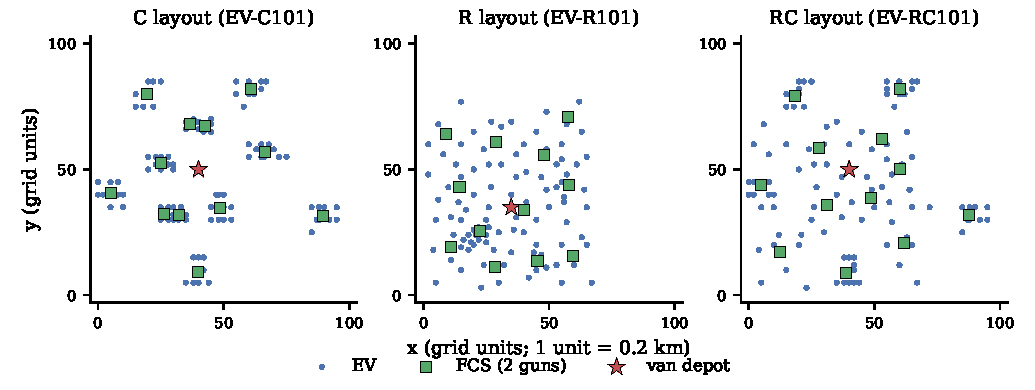
\includegraphics[width=\textwidth]{figures/instance_maps.pdf}
\caption{One instance of each layout (100 EVs, 12 FCS, 1 depot where all vans start and end).}
\label{fig:maps}
\end{figure}

\subsection{Demand: when EVs request and how much energy they need}

Pooling all EVs of all files in a family:
\begin{itemize}
  \item \textbf{When.} 17--27\,\% of the EVs request at minute 0 (Solomon files whose time windows were removed), and 68--85\,\% have requested by the middle of the day. Measured as a share of the day the six families look alike; the difference between the types is the length of the day. In type 1 the same 100 requests arrive within 230--240 minutes (R1, RC1), in type 2 within 960--3390 minutes, so type 1 is much more congested.
  \item \textbf{How much.} Energy is 10--40\,kWh in every layout and the same for types 1 and 2. C has many small demands (median 15.5\,kWh) and a few large ones; R and RC are spread more evenly (medians 17.4 and 19.2\,kWh). A demand of $E_i$ takes $60E_i/22$ minutes at an FCS and $60E_i/30$ minutes by van.
\end{itemize}

\needspace{8\baselineskip}
\subsection{What is taken from Solomon and what we added}

\begin{xltabular}{\textwidth}{@{}>{\raggedright\arraybackslash}p{4.6cm}>{\raggedright\arraybackslash}p{2.7cm}X@{}}
\toprule
\textbf{Solomon data} & \textbf{EV data} & \textbf{Rule} \\
\midrule
\multicolumn{3}{@{}l}{\textit{Taken from Solomon}} \\
Depot (customer 0) & van depot & unchanged; every van route starts and ends here \\
XCOORD., YCOORD. & EV locations & unchanged; 1 grid unit $=$ 0.2\,km, road distance $=1.3\times$ straight line \\
DEMAND (1--50) & energy $E_i$ & $E_i=10+30(\text{DEMAND}_i-1)/49$, i.e.\ 10--40\,kWh \\
READY TIME & request time $r_i$ & unchanged (minutes) \\
Depot DUE DATE & horizon $T$ & unchanged (minutes) \\
Travel rule & $t_{ij}$, $t_{if}$ & unchanged: 1 grid unit $=$ 1 minute, so $v=15.6$\,km/h \\
DUE DATE, SERVICE TIME & -- & not used; charging time is $\tau=60E_i/P$ \\
VEHICLE NUMBER, CAPACITY & -- & not used; replaced by the van fleet \\
\midrule
\multicolumn{3}{@{}l}{\textit{Added by us}} \\
-- & 12 FCS & 2 guns $\times$ 22\,kW each, at the $k$-means centres of the EV locations \\
-- & range $R_i$ & uniform on 5--40\,km; 15\,\% of the EVs are stranded (range 20--80\,\% of the distance to their nearest FCS) \\
-- & priority $w_i$ & $w_i=1+\kappa(1-R_i/R_{\max})$ with $\kappa=2$, so $w_i\in[1,3]$ \\
-- & 5 vans & $B_m=150$\,kWh, $Q_m=6$, $P^{\mathrm M}=30$\,kW, $\beta=0.25$\,kWh/km, $\eta=0.9$ \\
-- & costs (Rs) & $c^{\mathrm{EV}}=4$/km, $c^{\mathrm M}=15$/km, $c^{\mathrm F}_m=1500$/van, $\pi^{\mathrm F}=8.7$/kWh, $\pi^{\mathrm M}=10.7$/kWh, $c^{\mathrm W}=200/60$/min \\
\bottomrule
\end{xltabular}\addtocounter{table}{-1}

%=====================================================================
\section{Results}

Every one of the 56 files was solved with the complete model (1)--(20) in Gurobi for $n=10,20,\dots,100$ EVs (560 runs, at most 300\,s each, warm-started from a simple rule-based plan). Each run gives one row of \texttt{results.csv}. Every plan found was re-checked against all constraints and its cost recomputed independently.

\subsection{One instance in detail: EV-C101 with 10 EVs}

\begin{xltabular}{\textwidth}{@{}>{\raggedright\arraybackslash}p{4.6cm}>{\raggedleft\arraybackslash}p{2.9cm}>{\raggedright\arraybackslash}X@{}}
\caption{The result row of EV-C101 with $n=10$.}\label{tab:instance}\\
\toprule
\textbf{Column} & \textbf{Value} & \textbf{Meaning} \\
\midrule\endfirsthead
\toprule
\textbf{Column} & \textbf{Value} & \textbf{Meaning} \\
\midrule\endhead
\bottomrule\endlastfoot
\multicolumn{3}{@{}l}{\textit{Instance}} \\
instance & EV-C101\_n10 & file EV-C101, first 10 EVs \\
family & C1 & clustered layout, type 1 \\
EVs & 10 & number of charging requests $n$ \\
T\_min & 1236 & planning period $T$ (min) \\
stations / guns / vans & 12 / 24 / 5 & resources available \\
graph\_nodes & 23 & depot + 10 EVs + 12 stations \\
\midrule
\multicolumn{3}{@{}l}{\textit{Model size and solver}} \\
binaries & 843 & 0/1 variables $y,z,x,u,o$ \\
continuous & 10 & start times $S_i$ (one per EV) \\
constraints & 2278 & rows of (2)--(19) written out \\
build\_s & 0.07 & seconds to build the model \\
status & optimal & best plan found and proven best \\
Z\_Rs & 6119.56 & total cost $Z$ of the plan (Rs), recomputed by our checker \\
best\_bound\_Rs & 6119.56 & proven lower limit on $Z$; equal to $Z$, so nothing cheaper exists \\
gap\_\% & 0.0 & $100(Z-\text{bound})/Z$ \\
gurobi\_obj\_Rs & 6119.56 & Gurobi's own value of $Z$ (cross-check) \\
runtime\_s & 0.11 & solving time (s) \\
nodes\_explored & 1 & branch-and-bound nodes; solved at the root \\
greedy\_Z\_Rs & 7778.54 & cost of the rule-based starting plan \\
improvement\_vs\_greedy\_\% & 21.33 & saving of the MILP plan over the rule-based plan \\
valid & yes & plan meets every constraint \\
\midrule
\multicolumn{3}{@{}l}{\textit{Cost breakdown (Rs)}} \\
Z1\_EV\_drive & 12.30 & EVs driving to an FCS \\
Z2\_van\_drive & 176.23 & van kilometres \\
Z3\_dispatch & 1500.00 & one van dispatched \\
Z4\_energy & 1951.47 & energy at FCS and from the van battery \\
Z5\_inconvenience & 2479.56 & weighted waiting until fully charged \\
operating\_Z1\_to\_Z4 & 3640.00 & what the operator pays \\
total\_Z & 6119.56 & $Z_1+\dots+Z_5$ \\
\midrule
\multicolumn{3}{@{}l}{\textit{The plan}} \\
EVs\_at\_FCS / EVs\_by\_van & 4 / 6 & how the 10 EVs were served \\
vans\_used & 1 & of the 5 available \\
mean / max time to charged & 44.2 / 79.4 & minutes from request to fully charged \\
van\_km & 11.75 & total van distance \\
\end{xltabular}

\subsection{All 56 files: how far each one goes}

Table~\ref{tab:files} follows every file from 10 to 100 EVs.

% Generated by prepare_report.py from ../results.csv - do not edit here.
\begin{table}[H]
\centering\small
\caption{Outcome for every file over $n=10,20,\dots,100$ EVs. Plan up to: largest $n$ with a valid plan (-- = none). Optimal up to: every $n$ up to here proven optimal.}\label{tab:files}
\begin{tabular}[t]{@{}lrcc@{}}
\toprule
\textbf{File} & \textbf{$T$} & \textbf{Plan up to} & \textbf{Optimal up to} \\
\midrule
C101 & 1236 & 100 & 100 \\
C102 & 1236 & 100 & 30 \\
C103 & 1236 & 100 & 10 \\
C104 & 1236 & 100 & 10 \\
C105 & 1236 & 100 & 100 \\
C106 & 1236 & 100 & 90 \\
C107 & 1236 & 100 & 100 \\
C108 & 1236 & 100 & 100 \\
C109 & 1236 & 100 & 60 \\
\midrule
C201 & 3390 & 100 & 100 \\
C202 & 3390 & 100 & 60 \\
C203 & 3390 & 100 & 20 \\
C204 & 3390 & 100 & 20 \\
C205 & 3390 & 100 & 70 \\
C206 & 3390 & 100 & 70 \\
C207 & 3390 & 100 & 60 \\
C208 & 3390 & 100 & 70 \\
\midrule
R101 & 230 & 40 & 40 \\
R102 & 230 & 50 & 40 \\
R103 & 230 & 50 & 30 \\
R104 & 230 & 50 & 30 \\
R105 & 230 & 40 & 40 \\
R106 & 230 & 90 & 30 \\
R107 & 230 & 90 & 30 \\
R108 & 230 & 90 & 30 \\
R109 & 230 & 90 & 30 \\
R110 & 230 & 90 & 30 \\
R111 & 230 & 100 & 30 \\
R112 & 230 & 100 & 20 \\
\bottomrule
\end{tabular}
\hspace{1.5em}
\begin{tabular}[t]{@{}lrcc@{}}
\toprule
\textbf{File} & \textbf{$T$} & \textbf{Plan up to} & \textbf{Optimal up to} \\
\midrule
R201 & 1000 & 100 & 90 \\
R202 & 1000 & 100 & 70 \\
R203 & 1000 & 100 & 40 \\
R204 & 1000 & 100 & 30 \\
R205 & 1000 & 100 & 80 \\
R206 & 1000 & 100 & 60 \\
R207 & 1000 & 100 & 40 \\
R208 & 1000 & 100 & 30 \\
R209 & 1000 & 100 & 70 \\
R210 & 1000 & 100 & 70 \\
R211 & 1000 & 100 & 50 \\
\midrule
RC101 & 240 & 60 & 20 \\
RC102 & 240 & 60 & 20 \\
RC103 & 240 & 60 & 20 \\
RC104 & 240 & 100 & 20 \\
RC105 & 240 & -- & -- \\
RC106 & 240 & 70 & 20 \\
RC107 & 240 & 80 & 10 \\
RC108 & 240 & 80 & 10 \\
\midrule
RC201 & 960 & 100 & 50 \\
RC202 & 960 & 100 & 40 \\
RC203 & 960 & 100 & 30 \\
RC204 & 960 & 100 & 20 \\
RC205 & 960 & 100 & 40 \\
RC206 & 960 & 100 & 40 \\
RC207 & 960 & 100 & 40 \\
RC208 & 960 & 100 & 30 \\
\bottomrule
\end{tabular}
\end{table}


\end{document}
